% Chapter 1

\chapter{Introducción} % Introduccion al trabajo

\label{Chapter1} % For referencing the chapter elsewhere, use \ref{Chapter1} 

\lhead{Capítulo 1. \emph{Introducción}} % This is for the header on each page - perhaps a shortened title

%----------------------------------------------------------------------------------------

%--------------------------------------------------------
%Sección 1
%--------------------------------------------------------


\begin{figure}[htbp]
	\centering
		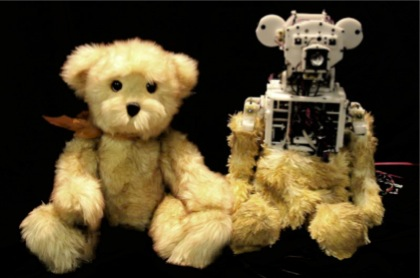
\includegraphics[width=0.8\textwidth]{./Figures/robot.jpg}
		%\rule{35em}{0.5pt}
%	\caption[Robot Huggable]{Robot creado por MIT Media Lab para cuidados personales. Imagen tomada de \cite{Stiehl:2006:HTR:1179133.1179149}}
	\label{fig:Huggable}
\end{figure}

El trabajo se centró en la investigación de las tecnologías existente para diseñar un robot que sea económico, simple y que de manera inalámbrica permita su control. El robot debe tener estas características ya que se necesita construir un enjambre para poder realizar estudios en el comportamiento y control de estos.

Al comienzo de este proyecto se trabajó en Santiago de Chile, en conjunto con la Universidad de Chile (UChile) bajo la tutela del Doctor Juan Cristóbal Zagal en el Laboratorio de Síntesis de Máquinas Inteligentes. Por parte de la Universidad Técnica Federico Santa María (USM), se trabajó con la Doctora María José Escobar, del Departamento de Electrónica y luego se incorporó el Doctor Pablo Prieto del Departamento de Diseño de Productos. El financiamiento para realizar este prototipo ha sido por parte de las dos Instituciones, Universidad Técnica Federico Santa María y Universidad de Chile.

Durante el proceso de desarrollo se tuvieron que hacer diversas compras de materiales, pero los lugares más recurrentes al momento de hacerlas fueron Olimex y Casa Royal. La primera es una empresa dedicada a traer productos para hacer prototipos y construir máquinas, la segunda cuenta con varios insumos básicos para trabajar en desarrollo de circuitos electrónicos. Ambas empresas se encuentran en Santiago, por lo que trabajar en esta ciudad es de gran ayuda para reducir los tiempos en desarrollo.
Luego de armar un primer robot funcional, con materiales disponibles en Santiago de Chile, se hizo una búsqueda en internet de componentes en tiendas especializadas.

Este documento resume el desarrollo del proyecto MODI (Modular Intelligence), que es un robot simple de construir que tiene como fin ser repetible para facilitar la construcción de Enjambres de robots. El capítulo 2 se explica lo que es un robot, algo de historia y algunos tipos de robots. El capítulo 3 comienza con un explicación sobre los enjambres de animales, luego se describen los robots usados actualmente en la literatura para estudiar enjambres y al final se describe las necesidades de mercado y las ventajas del proyecto MODI. El capítulo 4 está centrado en el diseño y herramientas de fabricación utilizadas durante el proceso de desarrollo. El capítulo 5 es el principal, describe criterios de diseño y el detalle de todos los componentes utilizados en el robot diseñado. Además se explica el software utilizado y el sistema que permite hacer un seguimiento de cada robot de forma individual. En el capítulo 6 se explican algunos posibles usos de los enjambres de robots. Al final, el capítulo 7 tiene sugerencias para mejoras futuras y las conclusiones.

%----------------------------------------------------------------------------------------